\chapter{Young Entrepreneur Interviews Millionaire Justin Waller}

This chapter is built from an interview rather than a blackboard lecture, but it still has a definite mathematical spine. The talk begins with scale and confidence, moves into the discipline of staying in one fight long enough to produce freedom, then turns to a simple but serious arithmetic of bootstrapping, leverage, debt service, and organizational design. We should therefore read it as a sequence: first the authority claim, then the allocation problem, then the financing problem, then the underwriting problem, and finally the problem of scaling human systems without losing ownership or initiative.

\section{Opening Stakes and the Interview Frame}

The source opens with a teaser montage: how much money has been made in a year, whether the speaker comes from money, whether he could rebuild from zero, and how a person becomes a multimillionaire. The host then resets in Miami and frames Justin Waller as a large construction operator. This is not yet the technical center of the lecture, but it establishes the promise that the later arithmetic is not abstract advice detached from operating experience.

Once the interview begins in earnest, the first concrete facts are about domain and duration. Waller says that he started in steel at age \(24\), that he has been in construction for roughly \(15\) years, and that the company now works coast to coast with more than \(200\) men. The important structural point is that the lecture does not begin with leverage or cap rates. It begins with the question of why one would stay in the same field long enough to earn the right to think about leverage at all.

\section{Staying in One Fight}

Waller's first serious claim is that the young self deserves credit for staying in the same fight. The contrast is not between work and laziness, but between depth and restless motion. People get hit a little, change directions, and then take the beginner's licks of the next industry. The alternative is to accept the pain of one field long enough to become dangerous in it.

The lecture's first model arrives almost immediately. We are told that freedom comes from concentration before diversification. First one stays in the same thing long enough to make substantial money. Only then does one go water other plants.

\subsection{Question \& Answer}

\paragraph{Question.} Why does concentration beat premature diversification?

\paragraph{Answer.} Because the scarce object is not opportunity in the abstract, but effective energy. If we keep resetting ourselves into beginner status, we do not compound skill, relationships, judgment, or operating leverage in any one domain. The interview's answer is not that diversification is bad forever. It is that diversification before mastery merely spreads weakness around.

A clean way to formalize the metaphor is to let total entrepreneurial energy be \(E\), and let the amount spent on project \(i\) be \(e_i\). Then
\begin{equation}
\sum_{i=1}^{n} e_i = E.
\end{equation}
This equation is editorial notation rather than spoken notation, but it captures the logic of the transcript exactly: energy is finite, and every new line of effort comes out of the same cup.

\begin{figure}[h]
\centering
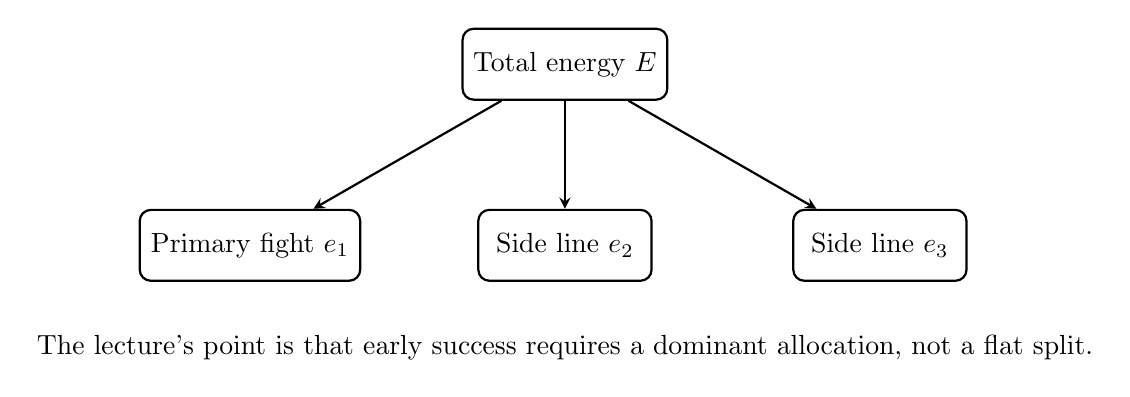
\begin{tikzpicture}[>=stealth, thick]
\node[draw, rounded corners, minimum width=2.6cm, minimum height=0.9cm] (E) at (0,0) {Total energy \(E\)};
\node[draw, rounded corners, minimum width=2.8cm, minimum height=0.9cm] (p1) at (-4,-2.3) {Primary fight \(e_1\)};
\node[draw, rounded corners, minimum width=2.2cm, minimum height=0.9cm] (p2) at (0,-2.3) {Side line \(e_2\)};
\node[draw, rounded corners, minimum width=2.2cm, minimum height=0.9cm] (p3) at (4,-2.3) {Side line \(e_3\)};
\draw[->] (E) -- (p1);
\draw[->] (E) -- (p2);
\draw[->] (E) -- (p3);
\node at (0,-3.6) {The lecture's point is that early success requires a dominant allocation, not a flat split.};
\end{tikzpicture}
\end{figure}

The talk does not give us a production function, and we should not invent one. But the intended conclusion is clear. If we pour too little into each plant, none bears fruit. If we produce freedom in one place first, later branching becomes a consequence of success rather than a substitute for it.

\begin{remark}
The water-and-plants model is the first real quantitative turn in the interview. It is not finance yet, but it is already an allocation problem.
\end{remark}

\section{Turning Point, Atmosphere, and the Next Mountain}

Only after the concentration argument is in place does the interviewer ask about background and turning point. Waller says plainly that he did not come from money and grew up in South Louisiana without money around him. The answer to the turning-point question is then given in a two-branch form: one either becomes the atmosphere one inhabits, or decides to be anything but that atmosphere.

This is less a numeric derivation than a statement of boundary conditions. The lecture wants us to see that ambition is not first born from formulas. It is born from a refusal of one equilibrium and a movement toward another. On that path, as he says, one finds more consciousness, and with each mountain climbed one searches for the next one. Happiness, in this telling, lives more on the ascent than at the peak.

The reason to keep this section in the notes is that the later arithmetic would otherwise sound bloodless. The interview's order matters. First a person rejects a limiting atmosphere, then he accepts concentration, then he earns freedom, and only then does he begin to discuss leverage, capital structure, and underwriting.

\section{Bootstrapping Without Cash}

The interview briefly pauses for a School of Mentors announcement, and then returns to the most practical question so far: how a business begins when there is not much money to start with. Waller's answer is operational rather than romantic. There was no money. He had to go win contracts, then take those contracts to the bank, and then try to obtain a line of credit against the existence of the business.

This is the first place where the lecture becomes crisp arithmetic. The first line of credit is given as
\begin{equation}
L_0 = \$15{,}000.
\end{equation}
The weekly payroll is given as approximately
\begin{equation}
P_{\text{week}} \approx \$2{,}500/\text{week}.
\end{equation}
He also tells us the scale of the operation: roughly two men, backyard buildings, and a business small enough that payroll itself is already a meaningful stress.

\subsection{Question \& Answer}

\paragraph{Question.} How do we finance a business before we have capital?

\paragraph{Answer.} The interview's answer is not ``wait until you are rich.'' It is: create evidence first, then borrow against the evidence. In this case the evidence is contracts already won. The bank does not finance a dream in the air; it finances the probability of cash flow.

\paragraph{Worked example.} If we isolate payroll alone and ignore materials, overhead, and receivables timing, then the first line of credit gives a rough payroll runway of
\begin{equation}
T_{\text{runway}} \approx \frac{L_0}{P_{\text{week}}}
\approx \frac{15{,}000}{2{,}500} \approx 6 \text{ weeks}.
\end{equation}
This should be read cautiously. It is not a full business valuation, nor even a full job-cost model. It is only a first bridge estimate. But that is precisely the spirit of the lecture: not elegance first, but enough arithmetic to survive the first few jobs.

We may summarize the spoken mechanism in four steps:
\begin{enumerate}
\item win contracts;
\item present those contracts to the bank;
\item obtain a credit line against that operating evidence;
\item use that credit line to carry payroll and execution until cash flow catches up.
\end{enumerate}

This is already a theory of entrepreneurial finance in miniature. Solvency is preferable, but if solvency is absent, the entrepreneur must manufacture a bridge.

\section{The Arithmetic of Real Estate}

The next question is the most explicit mathematical question in the interview: how to leverage capital, use good debt, and turn that into wealth. Here Waller moves from construction startup arithmetic into real-estate underwriting arithmetic. He says he owns more than \(400\) doors, and then names the core objects directly: net operating income, cap rate, debt service, and the cycle position of the property.

\subsection{Question \& Answer}

\paragraph{Question.} How does leverage create wealth without turning rate risk into a fatal blowup?

\paragraph{Answer.} The lecture's answer is that leverage is not magic and not pure courage. It is arithmetic plus timing. We must understand the property's income, the price paid for that income, the debt burden imposed on that income, and where we stand in the larger rate and cycle environment.

A standard clean notation for the spoken variables is
\begin{equation}
\mathrm{CapRate} = \frac{\mathrm{NOI}}{V},
\end{equation}
where \(V\) is the property value or purchase price, and
\begin{equation}
\mathrm{DSCR} = \frac{\mathrm{NOI}}{\mathrm{DS}},
\end{equation}
where \(\mathrm{DS}\) is annual debt service. The acronym \(\mathrm{DSCR}\) is editorial, but the logic is exactly the logic named in the interview: compare property income to required debt payments.

Waller also describes a simple capital stack: outside money for the down payment and long-term bank debt for the rest. In the most stripped-down notation,
\begin{equation}
C_{\text{stack}} = E_{\text{outside}} + D_{\text{bank}}.
\end{equation}
Again, the point is not sophistication for its own sake. The point is that a property purchase is assembled from components, and one must know what each component is doing.

The rate-risk warning is very concrete. He imagines a five- to seven-year ARM and asks what happens if a world that begins around \(7.5\%\) or \(8\%\) ends up resetting toward \(16\%\), as in a 1980-style scenario. In symbols, the stress he names is
\begin{align}
T_{\mathrm{ARM}} &\in [5,7] \text{ years},\\
r_0 &\approx 7.5\%\text{--}8\%, \qquad r_1 \approx 16\%.
\end{align}

A simple first-pass stress test, if we isolate the rate component on a fixed balance \(B\), is to note that the interest burden scales roughly with \(r\). So moving from \(r_0 \approx 8\%\) to \(r_1 \approx 16\%\) nearly doubles the rate component of debt service. This is not a full amortization model, but it is enough to explain the fear. If the income side does not move with the financing side, a once-comfortable property can become a problem property.

The interview's important rhetorical move is that, after naming this fear, Waller refuses mystification. He says the math is simple --- even ``third grade math.'' The real task is not advanced symbolism but disciplined attention: understand debt service, understand cycle position, pay attention to where rates may go, and leave yourself enough time to act before the reset becomes fatal.

\begin{remark}
The chapter should keep the formulas close to the spoken list of variables and should not pretend that a full underwriting spreadsheet is present in the source. The lecture gives us the governing objects, the governing risk, and the governing habit of mind.
\end{remark}

\section{Scaling from Seven Figures to Eight}

Later in the interview the host returns to annual earnings, clarifying both personal and business scale:
\begin{align}
M_{\text{take-home}} &\approx \$5\,\mathrm{M},\\
M_{\text{business}} &\approx \$35\,\mathrm{M}.
\end{align}
The next question is how the move from seven figures to eight figures happens. Waller's answer is not another asset formula. It is an organizational formula: systems, competent people, intent, ownership, autonomy, and aligned incentives.

Here the talk becomes almost algebraic in spirit, even if not in formal notation. We may write the core ingredients as
\[
S, \qquad K, \qquad I, \qquad O,
\]
where \(S\) denotes systems, \(K\) competence, \(I\) intent, and \(O\) ownership or autonomy. The causal sequence is what matters. A person may be skilled but not committed; committed but not capable; capable and committed but still detached if handed a plan in which he has no stake. The lecture therefore insists that staff should help build the systems they will later operate.

The sharpest image here is the negative one: a person who is handed a plan with no ownership sits in the boat with arms crossed, waiting for it to go wrong. That is the organizational analogue of passive capital. By contrast, if a person helps build the thing, he can get behind it. He can own it. And if he owns it, incentives can be written from the standpoint, ``I should be paying you more money,'' rather than, ``you should be making me richer.''

We should therefore read the seven-to-eight-figure discussion as a second leverage argument. The earlier leverage was balance-sheet leverage. This is human leverage. In both cases the key question is whether the structure amplifies performance or merely amplifies fragility.

\section{Scars, Repeatability, and the Rebuild Claim}

The closing movement returns to aphorism, but it does so after the arithmetic has already been laid down. The favorite mentor quote is that we can tell the size of a man by the size of his problems. Failure is reframed as material rather than interruption: the small bricks from which the castle is built.

This section matters because it closes the loop opened by the teaser. The claim that one could lose everything and make it back is not presented as raw bravado alone. It is grounded in repetition. If one keeps doing the same thing again and again, one acquires a superpower that is hard to confiscate. The operative asset is not only cash, not only property, not only contracts, but transferable competence in a domain.

That is why the lecture ends by returning to the same theme with which it began. The field matters. Staying in it matters. The scars matter. And the result is that the person becomes less dependent on a single current bank balance because the real capital has partly migrated into judgment, operating instinct, and repeatable action.

\section{Summary}

The interview proceeds in a clear order once we listen for its mathematics. First it establishes scale and authority. Then it argues for concentration: stay in one fight long enough to create freedom. Then it turns that into a resource-allocation model by treating energy as finite. After that it asks how a business begins without money, and answers with contracts, bank evidence, and credit. From there it moves into the arithmetic of real estate: \(\mathrm{NOI}\), cap rate, debt service, cycle timing, and ARM reset risk. Finally it translates financial leverage into organizational leverage through systems, competence, intent, ownership, and incentives.

The result is a chapter whose arithmetic is simple but not trivial. What appears again and again is the same pattern: do not diffuse scarce energy too early, do not mystify ordinary business math, and do not mistake scale for structure. The lecture's philosophy of resilience is therefore inseparable from its arithmetic. One can rebuild from zero only after one has learned what, exactly, is being compounded.